\chapter{Fonctionnement des caches}

Le but de cette partie est de résumer un certain nombre de techniques relatives à la gestion de la hiérarchie des caches. Nous commencerons par expliciter le comportement d'un cache en général, avant d'étudier les moyens mis en {\oe}uvre afin d'assurer la cohérence de l'ensemble des caches. Nous finirons par étudier les problèmes posés par la simulation des caches d'une architecture multi-c{\oe}urs, notamment le prefetching.

\section{Principes généraux d'un cache}
Cette section entend préciser le fonctionnement général d'un cache : comment il est possible d'y ajouter une donnée, quelle est la correspondance entre les blocs de la mémoire principale et les lignes de cache ou encore comment une donnée peut être evincée d'un cache. \\

Un cache possède un ensemble de sets contenant chacun un ensemble de lignes. Le nombre de lignes par set est appelé l'associativité du cache. Au chargement d'une donnée, elle est insérée dans une ligne vide du set correspondant à sa plage d'adresse. Les données qui suivent (dans la mémoire supérieure) la donnée voulue sont aussi recopiées afin de remplir totalement la ligne -- généralement de $32$ ou $64$ octets -- et exploiter le principe de localité spatiale (footnote ?).

\subsection{\'Etiquettes}
Pour pouvoir retrouver une donnée dans le cache, une table d'étiquettes est tenue à jour. Concrètement, une adresse mémoire est séparée en trois champs comme sur la figure suivante : \\

\begin{figure}[!h]
\begin{center}
   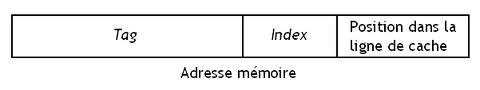
\includegraphics[scale=0.50]{etiquette.jpeg}
   \caption{\label{img:etiquette} Adresse mémoire}
\end{center}
\end{figure}

==> Préciser source de l'image\\

Le tag est stocké dans la table des étiquettes, il servira a identifier les différents blocs mémoires pouvant être au même endroit dans un cache. L'index correspond au numéro de set dans lequel se trouve la ligne de cache. Pour finir l'offset correspond au bloc dans la ligne de cache.

\subsection{Fonction de correspondance}
Un cache de taille $n$ contient un ensemble $p$ de lignes de taille $m$, tel que $n = p \times m$. Afin de placer et récupérer une donnée dans le cache, une fonction de correspondance avec la mémoire est nécessaire. Il existe trois cas de figure. Pour la suite, nous prendrons : \\
\begin{itemize}
\item $i$ le numéro de set du cache
\item $j$ le numéro du bloc mémoire
\item $s$ le nombre de sets du cache
\item $k$ l'associativité du cache 
\end{itemize}

\subsubsection{Direct associative}
Un cache est en correspondance directe si à chaque bloc mémoire est associé une unique ligne du cache. Le nombre de sets, $s$, du cache est alors égal à son nombre de lignes, $p$. Lorsqu'un bloc mémoire $j$ est ajouté dans le cache, la ligne correpondante est chargée à la ligne $i = j\ modulo\ s$. Avec ce type de cache, il est facile d'ajouter ou de retrouver une données. Cependant, si plusieurs blocs mémoires correpondant à la même ligne de cache sont fréquemment utilisés, il faudra sans cesse supprimer et ajouter des données dans le cache.

\subsubsection{Fully associative}
Un cache est en correspondance associative si chaque bloc mémoire peut être mis dans n'importe quelle ligne du cache. Il n'y a alors qu'un seul set. L'inconvénient précédent n'est plus existant, cependant il devient beaucoup plus compliqué de rechercher une donnée dans le cache. L'ensemble des étiquettes doit en effet être parcouru.

\subsubsection{$k$-ways associative}
Les deux cas présentés précedemment présentent des inconvénients. Généralement, un cache profite des avantages des deux visions en faisant un compromis. Dans le cas de la correspondance associative par ensemble, chaque set possède un nombre $k$ de lignes tel que $p=k \times s$. La fonction de correspondance est telle que $i = j\ modulo\ s$. De cette manière, un bloc mémoire peut se trouver dans un ensemble de $k$ lignes. Il est donc possible d'avoir plusieurs blocs mémoires correspondant au même ensemble et l'algorithme de recherche est plus efficace que dans le cas de la correspondance associative.

\begin{figure}[!h]
\begin{center}
   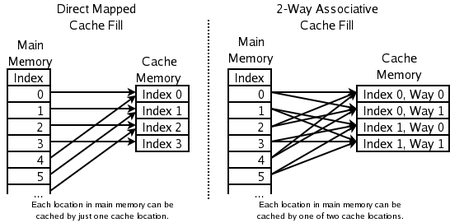
\includegraphics[scale=0.60]{associative.png}
   \caption{\label{img:associative} Fonction de correspondance}
\end{center}
\end{figure}

==> Préciser source de l'image\\

\subsection{Politiques de remplacement}
 Lorsque l'on souhaite ajouter une ligne dans un set plein, il faut au préalable évincer une ligne de ce set. Pour cela, il existe différentes méthodes :

\paragraph{FIFO.} La première solution consiste à supprimer la ligne la plus ancienne du cache. Cela correspond à la formule: ``First In, First Out''.

\paragraph{LFU.} Une autre solution consiste à supprimer la ligne qui a été le moins utilisée: ``Least Frequently Used''. Pour cela, chaque ligne de cache possède un compteur qui sera incrémenté à chaque utilisation de la ligne. 

\paragraph{LRU.} La dernière solution, généralement utilisée, consiste à favoriser le principe de localité temporelle en supprimant la ligne du set qui a la plus ancienne date d'utilisation: ``Least Recently Used''.

\newpage
\section{Gestion de la cohérence}
Dans les systèmes actuels, un processeur n'est plus composé d'un unique c{\oe}ur, mais de plusieurs. Chaque c{\oe}ur possède généralement deux caches qui lui sont propres : le L1i pour stocker les instructions et le L1d pour stocker les données. Les caches de niveau supérieur sont quant  eux partagés par un nombre variable d'autres caches (et c{\oe}urs). Alors que les interactions entre ces deux premiers caches sont minimes -- il est difficile de mélanger instructions et données --, la cohérence entre les autres est en revanche un problème de taille.

\subsection{Présentation du problème}
Les caches sont utilisés à chaque \textit{load}/\textit{store}. S'il est possible que plusieurs caches possèdent la même donnée et la lisent en même temps, il est primordial qu'une donnée ne puisse pas être modifiée simultanément dans deux caches. Pour cela, des techniques hardware(mettre du français ?) sont mises en place afin de définir qui a la priorité si plusieurs c{\oe}urs veulent modifier une même donnée. \\

Par ailleurs, un protocole de cohérence est mis en {\oe}uvre à chaque \textit{load}/\textit{store} afin que les différents caches soient informés des modifications les concernant et que la consistance du système soit assurée. Ce protocole est propre à un niveau de cache. Dans un cas classique, il y aura un protocole de cohérence entre les L1 et entre les L2.

\subsection{Protocoles de cohérence}
 Nous étudierons uniquement le protocole de type MSI et ses dérivés : MESI, MOSI et MOESI. Chaque ligne de cache possède un état qui permet de gérer la cohérence. Les différents états sont: \\
\begin{itemize}
\item M: Une ligne est dans l'état modifié si c'est la seule copie valide dans l'ensemble des caches du niveau. Dans ce cas, si la ligne est evincée du cache, elle doit être recopiée en mémoire, via un write back. \\
\item S: Une ligne est dans l'état partagé (\textit{shared}) si elle est valide et qu'elle n'a pas été modifiée. Dans ce cas, plusieurs caches peuvent possèder la ligne. \\
\item I: L'état invalide est utilisé pour une ligne qui n'est pas valide. Le contenu de la ligne n'étant pas viable, il ne faut pas l'utiliser. \\
\item E: Une ligne est dite exclusive si elle est, dans le niveau, la seule copie valide. Une ligne dans cet état n'a pas été modifiée et les données de la ligne sont identiques à celles de la mémoire principale. \\
\item O: L'état \textit{owned} est utilisé pour un cache qui possède une donnée invalide dans la mémoire principale. Plusieurs caches peuvent possèder la même donnée, ils seront alors dans l'état S. \\
\end{itemize}

L'état M est utilisé lorsque la donnée a été modifiée par un c{\oe}ur. Il existe deux cas de propagation des modifications. Dans le choix de la politique \textit{write-through}, la donnée est directement recopiée dans la mémoire principale pour éviter de futurs problèmes de cohérence. Dans le cas de la politique \textit{write-back}, la donnée est modifiée uniquement dans le cache. Les autres caches et la mémoire principale peuvent savoir que la donnée a été modifiée, en revanche ils n'ont pas la dernière copie valide. Ils peuvent l'obtenir lors des \textit{Write-Back}: lorsque la donnée est evincée du cache ou lorsqu'elle est demandée à un plus haut niveau pour des soucis de cohérence.\\

Le protocole de cohérence le plus utilisé est MESI. Voici certaines caractéristiques de ce protocole : \\
\begin{itemize}
\item Lorsqu'un cache charge une donnée, il demande si un autre cache possède la donnée. Si un cache possède la donnée dans l'état M, alors ce cache fait un Write-Back et invalide sa donnée. Si un autre cache possède la donnée en état E, la donnée passe dans l'état S pour les deux caches. Si plusieurs (ou un seul) caches possèdent la donnée dans l'état S, la donnée est ajoutée dans l'état S.
\item Si un cache possède une donnée dans l'état M ou E et fait un nouveau \textit{store} sur la ligne de cache, son état devient M et aucune information n'est transmise aux autres caches.
\item Si un cache fait un \textit{store} sur une donnée qui est dans l'état S, la même donnée est invalidée dans les autres caches du même niveau. \\
\end{itemize}

Le protocole est souvent représenté sous la forme d'un automate, dont les états possibles sont ceux des données : \\

\begin{figure}[!h]
\begin{center}
   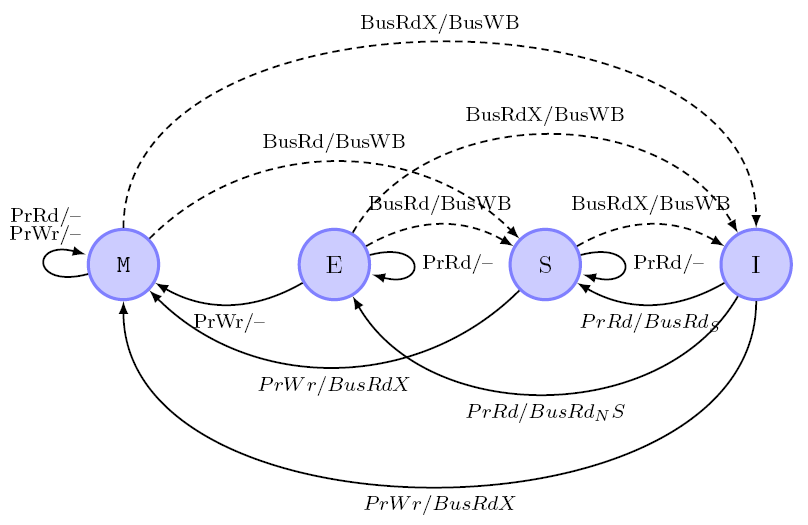
\includegraphics[scale=0.45]{mesi.png}
   \caption{\label{img:mesi} Automate du protocole MESI}
\end{center}
\end{figure}

==> Préciser source de l'image + légende\\

Pour l'état O, la différence est que les interactions avec la mémoire principale sont moins importantes. En effet, lorsqu'un cache qui n'a pas la donnée fait un \textit{load}, le cache possédant la donnée dans l'état O peut lui donner sans faire de \textit{write-Back}. Cela permet de garder plus longtemps la donnée modifiée.

\newpage
\section{Fonctionnement global}
La cohérence expliquée jusqu'à présent correspondait à celle d'un niveau de caches. Mais il peut arriver d'autres problèmes de gestion des données entre ces différents niveaux car les niveaux de caches peuvent être inclusifs, exclusifs ou non-inclusifs. Par ailleurs, les particularités du snooping, qui consiste à demander via un bus une donnée aux autres caches du même niveau, seront aussi explicitées. \\

Le cas inclusif est plutôt orienté \textsc{Intel} alors que le cas exclusif est plutôt mis en place par \textsc{AMD}. De son côté \textsc{ARM} oscille entre les deux solutions proposées.

\subsection{Caches inclusifs}
Le fonctionnement d'un cache inclusif est relativement simple. En cas de \textit{hit}, la donnée est propagée au cache (ou au processeur) qui a préalablement demandé la donnée. En cas de \textit{miss}, une demande de donnée est effectuée au niveau du dessus. La donnée est ensuite propagée à la mémoire d'en dessous. Dans le cas d'une hiérarchie avec uniquement des caches inclusifs, les messages utilisés pour demander/donner les données se font uniquement de façon verticale dans la hiérarchie. Il y a parallèlement, des messages destinés à garantir la consistance du système qui sont gérés différemment et qui influent sur la totalité de la hiérarchie. Voici un résumé des messages envoyés dans le cas d'une demande de donnée, en ne tenant pas compte de la gestion de la cohérence : \\

\begin{figure}[!h]
\begin{center}
   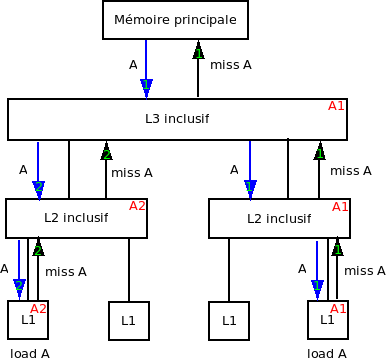
\includegraphics[scale=0.7]{inclusifs.png}
   \caption{\label{img:inclusifs} Caches de niveau 2 et 3 inclusifs}
\end{center}
\end{figure}

==> Préciser source de l'image + légende\\

D'un point de vue de la simulation, il est utile de modéliser les messages partant du bas de la hiérarchie (les caches L1) et remontant jusqu'à la mémoire principale. Le caractère inclusif prend tout son intérêt : la recherche est simple et la gestion de la cohérence séparée des échanges bruts de données, qui demandent plus de bande passante.\\

==> Pas clair (On parle ici de généralité sur les caches, il ne faudrait pas garder ça pour "notre" partie ?)

\subsection{Caches exclusifs}
Cependant, le fait qu'un cache soit inclusif pose un problème : les données sont dupliquées dans la hiérarchie. De ce fait, la taille réellement utilisable de l'ensemble des caches est en fait inférieure à la taille théorique. Les caches exclusifs ont justement pour principal objectif de limiter cette duplication des données. Par exemple, si un L2 est exclusif, les L1 en dessous ne pourront pas contenir une donnée déjà présente dans le L2, et inversement. Concrètement, il y a quatre cas de figure : \\

==>un joli schéma\\
\begin{itemize}
\item Si un L1 fait un \textit{hit}, il transmet la donnée au c{\oe}ur associé
\item Si un L2 fait un \textit{hit}, il donne la donnée au L1 qui l'a demandé puis la supprime.
\item Si un L1 fait un \textit{miss}, il effectue une demande de donnée au L2 associé. Il gardera la donnée une fois qu'elle lui sera transmise.
\item Si un L2 fait un \textit{miss}, il effectue une demande de donnée au L3 associé, ou directement à la mémoire principale si il n'y a pas de L3. Une fois que la donnée lui sera transmise, il la propagera au L1 sans la conserver. \\
\end{itemize}

Il en va de même pour les interactions entre les L2 et les L3, voire d'autres niveaux dans le cas d'une architecture plus grande. Par ailleurs, lorsque le dernier niveau fait un \textit{miss}, il faut parcourir l'ensemble de la hiérarchie avant de rechercher directement la donnée dans la mémoire principale. Ce phénomène explique à lui seul le fait que la gestion de la recherche et de la cohérence soit plus délicat que dans le cas d'une hiérachie avec le dernier niveau inclusif.

\subsection{Caches non-inclusifs}
Il existe un autre cas de figure, qui peut être considéré comme une variante du cas exclusif. Lorsqu'un L1 demande une donnée et que le L2 ne l'a pas, il se contentera de propager la donnée sans la conserver en mémoire. Cependant, si il avait préalablement la donnée, il la propagera au L1 sans pour autant la supprimer. Ce cas de figure peut être utilisé pour un L2 avec un L3 inclusif. De cette manière, la hiérarchie permet en moyenne de stocker plus de blocs mémoires sans pour autant compliquer la gestion de la cohérence. \\

Un autre cas de figure est un cache non-inclusif qui fonctionne avec plus de souplesse qu'un cache inclusif. Les données sont toujours laissées au passage, par contre l'inclusivité n'est pas formelle: il peut perdurer dans un L1 une donnée qui a été ejectée d'un L2 par exemple.

\subsection{Ajout du snooping}
 Il est possible que les caches d'un même niveau soient reliés ensemble par un bus. La méthode de recherche sur ce bus est alors appelée snooping. Prenons l'exemple d'une hiérarchie à trois niveaux où les L2 seraient reliés par un bus. Lorsqu'un L1 fait un \textit{miss}, il demande au L2 associé de lui fournir la donnée. En cas de nouveau \textit{miss}, la demande est envoyée en broadcast sur le bus afin de récupérer la donnée sans passer par le L3. Si aucun cache ne possède la donnée, la demande est alors transmise au L3.

\newpage
\section{Comportements spéciaux}
Les politiques de remplacement, de cohérence et les différents types de caches offrent un ensemble de modularités dans la gestion d'une hiérarchie de caches. Cependant, d'autres possibilités existent afin d'améliorer les performances de l'ensemble.

\subsection{Utilisation d'un \textit{victim cache}}
Généralement, des caches à $k$ voies associatifs sont utilisés, car la fonction de recherche d'une donnée est peu coûteuse et plusieurs blocs mémoire correspondant à un même set peuvent être stocké dans un cache. Dans la plupart des cas, le nombre de voies varie entre $2$ et $12$. \\

Dans certains cas, il est possible que le nombre de voies ne soit pas suffisant car un ensemble de blocs mémoire correspondant au même set est très utilisé. Cela est notamment vrai pour les L1 qui possèdent généralement peu de voies. Pour pallier ce problème et limiter les échanges de données entre les L1 et les L2, il est possible d'utiliser un buffer pour stocker les victimes d'éviction. Ce buffer est de petite taille, par exemple $8$ fois la taille d'une ligne de cache. De cette manière, lorsqu'un donnée est supprimée du L1, elle est placée dans le buffer correspondant. Lorsque le L1 fait un \textit{miss}, il commence par regarder dans le buffer (le coût est alors faible). Les données arrivant dans le L2 sont alors celles evincées du buffer.

\subsection{Suivi des données}
 Il existe différentes manières de localiser les données dans une hiérarchie mémoire -- il ne s'agit pas ici de la recherche au sein d'un cache, cela est géré par la table d'étiquettes, mais bien entre les caches. Deux cas fréquents se posent, ils sont réglés la plupart du temps par un \textit{tracking} : dans quels caches se trouvent les données.

\subsubsection{Supprimer les données}
Lorsqu'un cache L1 utilise une donnée qu'il possède déjà dans son cache, les flags utilisés par les politiques de remplacement sont mis à jour afin de supprimer les bonnes données lorsqu'un set sera plein. Cependant, les caches de plus haut niveau (L2, L3) ne sont pas mis au courant que la donnée a été utilisée et ils ne changent donc pas les flags de remplacement. Ainsi, lorsque le L2 aura un set plein, il se peut qu'il supprime une donnée très utilisée dans un L1. \\

Dans le cas d'un cache inclusif, il faut donc, à la suppression d'une donnée, invalider la donnée dans les caches en dessous afin de conserver le caractère inclusif. Pour limiter ce problème, les L2 et les L3 peuvent suivre les données, c'est-à-dire posséder une table indiquant quels caches de niveau plus bas ont également la donnée. De cette manière, les politiques de remplacement peuvent être adaptées en définissant des priorités: par exemple, éviter de supprimer les données qui sont contenues dans beaucoup de caches.

\subsubsection{Savoir qui a les données}
Dans le cas d'un cache de dernier niveau et exclusif, s'il se produit un \textit{miss}, il faut parcourir l'ensemble de la hiérarchie avant d'évenetuellement faire appel à la mémoire principale. Cela pose des problèmes, tant au niveau de la recherche des données que de la gestion de la consistance du système. Pour pallier ce problème, le cache de dernier niveau peut être lié à un table d'étiquettes, permettant de savoir quelles sont les données contenues dans chaque cache. Cela évite d'avoir à parcourir l'ensemble de la hiérarchie mais il y a un coût en terme de mémoire. Cependant, ce coup est faible (les données ne sont pas stockées) et bien inférieur au coût mémoire de la duplication dans le cache d'un cache de dernier niveau inclusif.
